% pick and place is almost every problem
% however, some objects are located at pick is not impossible (although the object is pick able)
% at this time, we should rearrange the object with non-prehensile motion and make the object prehensile able.
% and then manipulate with diverse 

How can a robot sequence skills to manipulate objects when the objects are in a configuration that is difficult to manipulate? For instance, consider the task of flipping a thin card placed in the middle of a table, as shown in the top row of Fig. \ref{fig:CPNP_tasks}. Since the card is not directly graspable, the robot should first push the card to the end of the table, flip it and return it to the center of the table. Such a task requires not only determining which manipulation skills are feasible based on the current state but also building a long-term skill plan that considers the functional relationships between skills. This is a challenging problem that includes highly stochastic state transitions arising from contact-rich manipulations while finding valuable subgoals that will enable applying the subsequent skill and eventually lead to task success.

% add the skill libarary
There are two conventional approaches to solving these kinds of problems. The first line of work formulates the problems as Parameterized Action Markov Decision Processes (PAMDPs) \cite{hausknecht2015deep,jain2020generalization, jiang2024hacmanpp, masson2016reinforcement,  nasiriany2022augmenting, wei2018hierarchical, xiong2018parametrized, li2021hyar}. In this formulation, skills are parameterized by a discrete action and corresponding continuous parameters, such as an index for a grasping skill and its position. A high-level policy is learned to flexibly select skills and its parameters from a reward signal using reinforcement learning (RL).
However, this approach requires a well-defined, task-specific reward function to mitigate the exploration and credit assignment problems of RL, which hinders the algorithms' applicability in long-horizon tasks. 

% Moreover, the transition of their skills is feasible in most states, which limits the range of tasks where viable state space of skills is restricted such as card picking being available if and only if it is at the end of a table.

% TODO 
Another approach is task and motion planning (TAMP) \cite{garrett2021integrated}, which is a class of planning problems that involve discrete task planning and continuous motion planning, analogous to our problem of finding discrete skills and continuous skill subgoals. Although TAMP algorithms have been demonstrated in solving long-horizon problems, they are typically not favored for real-world applications. The primary reasons are the high computational cost—often causing robots to wait about a minute before execution—and the need for re-planning when unexpected state transitions occur. These challenges are especially pronounced in contact-rich manipulation tasks due to the inherent uncertainty of real-world dynamics. Despite these limitations, we prefer to adopt TAMP-like algorithms for their capability to solve long-horizon problems.

% they require symbolic representations of domain-specific knowledge—such as whether an object is graspable—to solve the problem in a reasonable time, which is a strong assumption and often impossible to obtain in the real world. Moreover, the accurate design of preconditions, effects, and constraints of operators is necessary, making the application of complex RL based skills uncertain.
%One way to solve this problem is first finding a plan skeleton without specifying continuous parameters and fill out and refine the parameters with sampling or optimization.
% TAMP needs accurate modeling.


% Cannot get predicate in real-world
% Assume symbolic state transition (or mode changes) is deterministic in task planning. Do not take into account a stochastic mode transition such as miss the object during grasping might due to stochastic skill policy or real-world dynamics. We combat with such stochastic with actually simulate the skill and dynamcis i.e. effect of action operator may not be satisfied. stochastic making and breaking contact.
% Quasi-static assumption -> if not hold, what happen? mode changes during action operater?
% Do not model skills as TAMP action as precondition and effect cannot be figured out in neural network (NN) policy.
% Skeleton first search, and continous params later. This approach cannot perform geometrical reasoning or need another predicates to efficiently solve the problem. For example, it is impossible to reason whether the card is graspable before specifying subgoal. To make it efficient, domain-specific predicates such as a knowledge of graspable object region is required.
% Modeling skill effect is too difficult (e.g. how robot configurations looks like after pushing)
% Symbolic representation of complex geometric and kinematics requires human engineering
% We propose simple yet effective algorithm that find a sequence of skills and subgoals.

% Explain SKill-RRT here.
To address contact-rich skill-chaining problems, we propose a two-stage framework: (1) demonstration generation in simulation and (2) imitation learning (IL). In the first stage, we generate successful state-action trajectories using a simple yet effective skill-planning algorithm called \texttt{Skill-RRT}, which is based on the rapidly-exploring random tree (RRT) algorithm \cite{lavalle1998rapidly}. \texttt{Skill-RRT} can chain various skills for a given random initial state and goal without assuming that the skill skeleton is known. After collecting diverse trajectories, we distill the demonstrations into a single IL policy because \texttt{Skill-RRT} is not suitable for direct application in the real world, as described earlier. A single IL policy facilitates real-time execution through feedforward action prediction for a given state, eliminating the need for exhaustive planning.

\texttt{Skill-RRT} is a skill planning algorithm that finds a sequence of skills and their subgoals for a given initial state and goal. It is designed to eliminate the necessity for task-specific reward functions and to reduce the effort of hand-designing domain descriptions. Skills trained using RL are first formulated with given preconditions and effects, similar to the operators in TAMP, which are simply defined based on an object pose and a robot configuration. Using these skills, \texttt{Skill-RRT} attempts to extend a tree towards randomly sampled nodes, including subgoals, via their associated skills. The connectivity (or feasibility) between the nearest node in the tree and the random node is checked by the skill's precondition—such as whether the skill can achieve the subgoal given the nearest object pose and robot joint configuration—and then by actually executing the skills in simulation. If the skills succeed, the sampled node is appended to the tree, and the algorithm continues to explore other nodes to reach the given goal. This algorithm is advantageous because it requires little knowledge of skills and domain (e.g. regions of collision-free object poses), thereby eliminating the need for complex skill models \cite{liang2022search} or engineered heuristics \cite{barry2013hierarchical}.

%We compare our methods with existing works in Table. \ref{table:baseline_comparison}

Even though \texttt{Skill-RRT} can effectively chain multiple skills, the existing skills do not always guarantee task success. This is primarily because the effects of the preceding skills and the preconditions of the subsequent skills typically do not align. For instance, consider a scenario where a robot pushes a card to the edge of a table and maintains contact with the card (illustrated in the first column of the first row in Fig. \ref{fig:CPNP_tasks}). The next skill would be a place skill (depicted in the third column of the first row in Fig. \ref{fig:CPNP_tasks}), so the robot needs to be in a grasping location, but these two states are not identical. Therefore, we need an intermediate skill that moves the robot to the desired grasping location, which would not be present in our current skills. While one may consider utilizing a motion planner to generate such motion, it cannot effectively transition between the two states because modeling the dynamics of making and breaking contact between the robot and the object is often impossible. Consequently, the motion planner could cause the object to move, resulting in the object no longer being graspable or causing it to fall off the table. For that reason, we require intermediate skills, called connectors, that robustly chain the effect of the former skill and the precondition of the following skill, but we do not know which skills should be chained until we establish skill plans.

 
To decide which skills to chain, we divide \texttt{Skill-RRT} into two levels inspired by \cite{kaelbling2011hierarchical}: abstract and full. The \texttt{Abstract Skill-RRT} generates abstract plans with existing skills optimistically assuming that the state differences between the skills' effects and preconditions can be transferred. Since assuming that any states can be transferred to other states is unrealistic and a strong assumption, we add a minimal condition related to object poses. More concretely, if the final object pose of the previous skill matches the object pose precondition of the subsequent skill, we assume that a single connector can adjust the robot configuration to satisfy the precondition (e.g. grasping a card) without causing object movement that might lead to deviation from the precondition. In this way, connector problems can be collected without constructing full skill plans, and the collected problems are more focused on task-related states. The connectors are then trained using an off-the-shelf RL algorithm such as Proximal Policy Optimization (PPO) \cite{schulman2017proximal} and full \texttt{Skill-RRT} searches skill plans to solve a given problem.

\documentclass[border=0pt]{standalone}
\usepackage{pgfplots}
\pgfplotsset{width=\linewidth,compat=1.8}
\usepackage{amsmath}
\usepackage{pgfplotstable}
\usepgfplotslibrary{fillbetween}
\providecommand{\datapath}{.}


\pgfplotsset{every tick label/.append style={font=\boldmath\Huge}}
\tikzstyle{every node}=[font=\bfseries\Huge]

\begin{document}
\pgfplotstableread[col sep=comma,]{\datapath/dcfr9_2.csv}\dcfrb
\pgfplotstableread[col sep=comma,]{\datapath/dcfr16_2.csv}\dcfra
\pgfplotstableread[col sep=comma,]{\datapath/cams_2.csv}\cams
 \LARGE
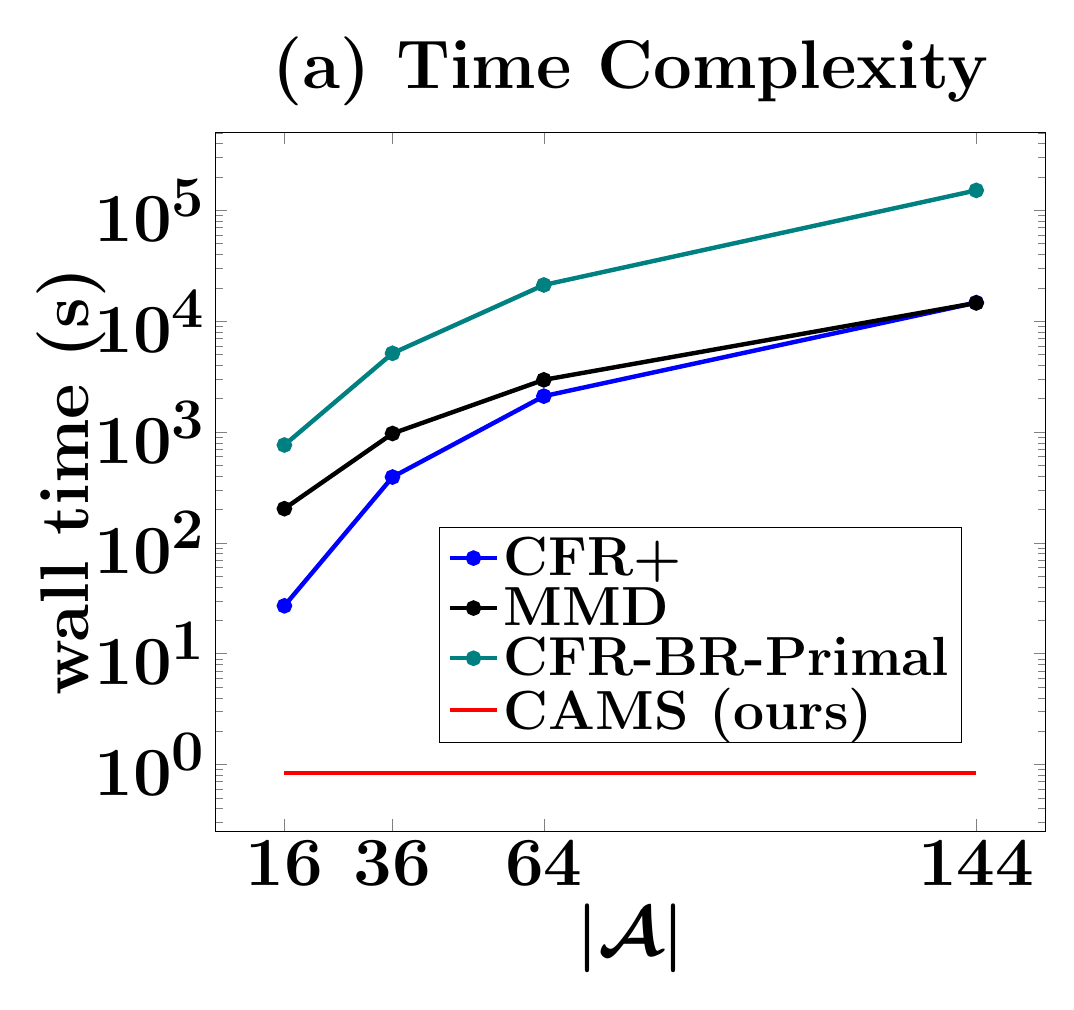
\begin{tikzpicture}[scale=1]
\begin{axis}[title={(a) Time Complexity},
    legend style={nodes={scale=0.8}, style={at={(0.9, 0.435)}}, fill=none},
    legend cell align={left},
    legend entries={CFR+, MMD, CFR-BR-Primal, CAMS (ours)},
    xlabel={$\boldsymbol{|\mathcal{A}|}$},
    ylabel={\textbf{wall time (s)}},
    xtick={16, 36, 64, 144},
    ymode=log,
    % xmode=log,
    ylabel shift=-11pt,
]
% cfr+
\addplot [mark=*, mark size=2pt, ultra thick, blue] coordinates {
(16, 27.05)
(36, 392.77)
(64, 2108.81)
(144, 14707.94)
};
%mmd
\addplot [ultra thick, black, mark=*, mark size=2pt] coordinates {
(16, 203.58)
(36, 970.45)
(64, 2958.36)
(144, 14629.44)
};
%cfr-br-primal
\addplot [ultra thick, teal, mark=*, mark size=2pt] coordinates {
(16, 764)
(36, 5136)
(64, 21238)
(144, 151596)
};
% cams
\addplot [ultra thick, red] coordinates {
(16, 0.842)
(36, 0.842)
(64, 0.842)
(144, 0.842)
};

\end{axis}
\end{tikzpicture}%
% iterations count
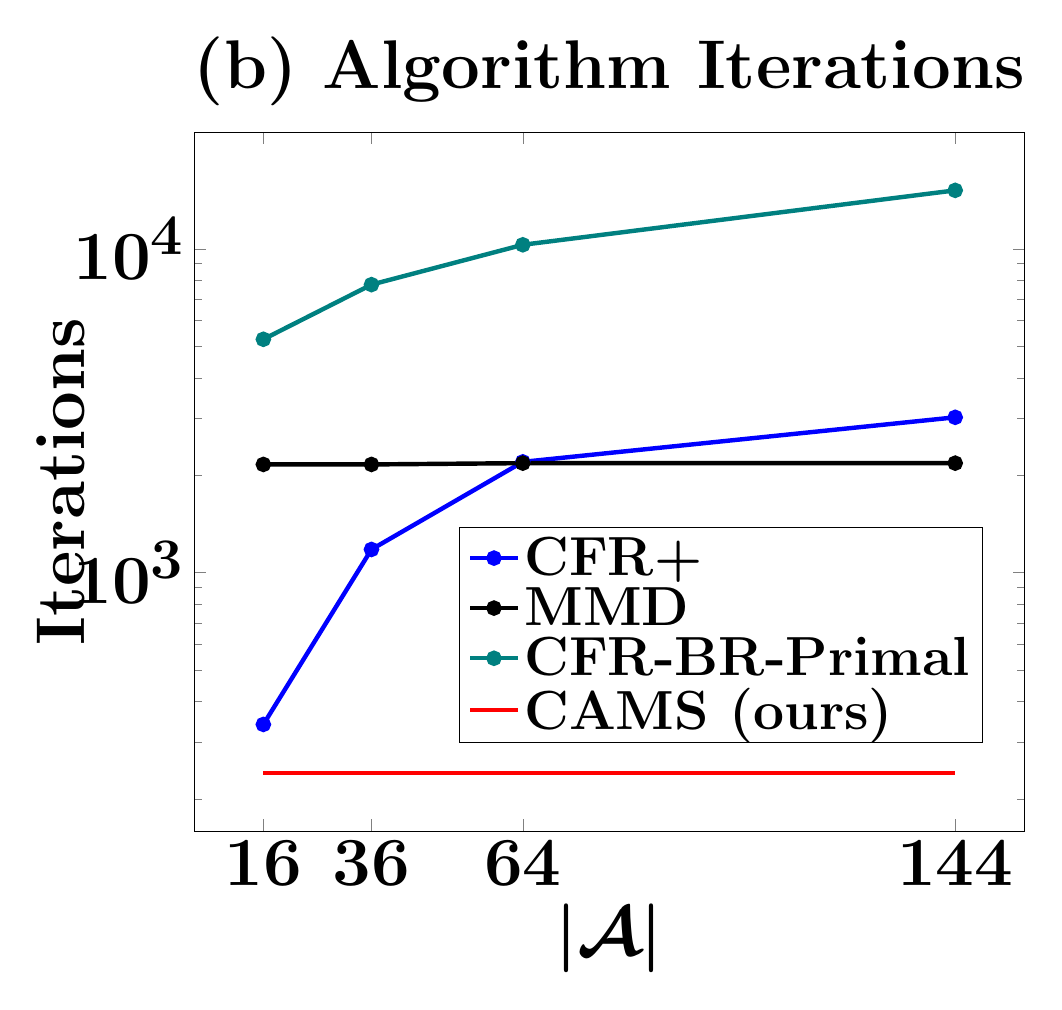
\begin{tikzpicture}[scale=1]
\begin{axis}[title={(b) Algorithm Iterations},
    legend style={nodes={scale=0.8}, style={at={(0.95, 0.435)}}, fill=none},
    legend cell align={left},
    legend entries={CFR+, MMD, CFR-BR-Primal, CAMS (ours)},
    xlabel={$\boldsymbol{|\mathcal{A}|}$},
    ylabel={\textbf{Iterations}},
    xtick={16, 36, 64, 144},
    ymode=log,
    ylabel shift=-11pt,
    % ytick distance=10^.4,
    % log ticks with fixed point,
    % ymin=1e1,
    % ytick={150, 1000, 7000},
    % ytick = {1, 10^1, 10^2, 10^3},
]
% cfr+
\addplot [mark=*, mark size=2pt, ultra thick, blue] coordinates {
(16, 340)
(36, 1180)
(64, 2200)
(144, 3020)
};
%mmd
\addplot [ultra thick, black, mark=*, mark size=2pt] coordinates {
(16, 2160)
(36, 2160)
(64, 2180)
(144, 2180)
};
% cfr-br-primal
\addplot [mark=*, mark size=2pt, ultra thick, teal] coordinates {
(16, 5260)
(36, 7760)
(64, 10300)
(144, 15169)
};
% cams
\addplot [ultra thick, red] coordinates {
(16, 241)
(36, 241)
(64, 241)
(144, 241)
};

\end{axis}
\end{tikzpicture}%
% distance to gt
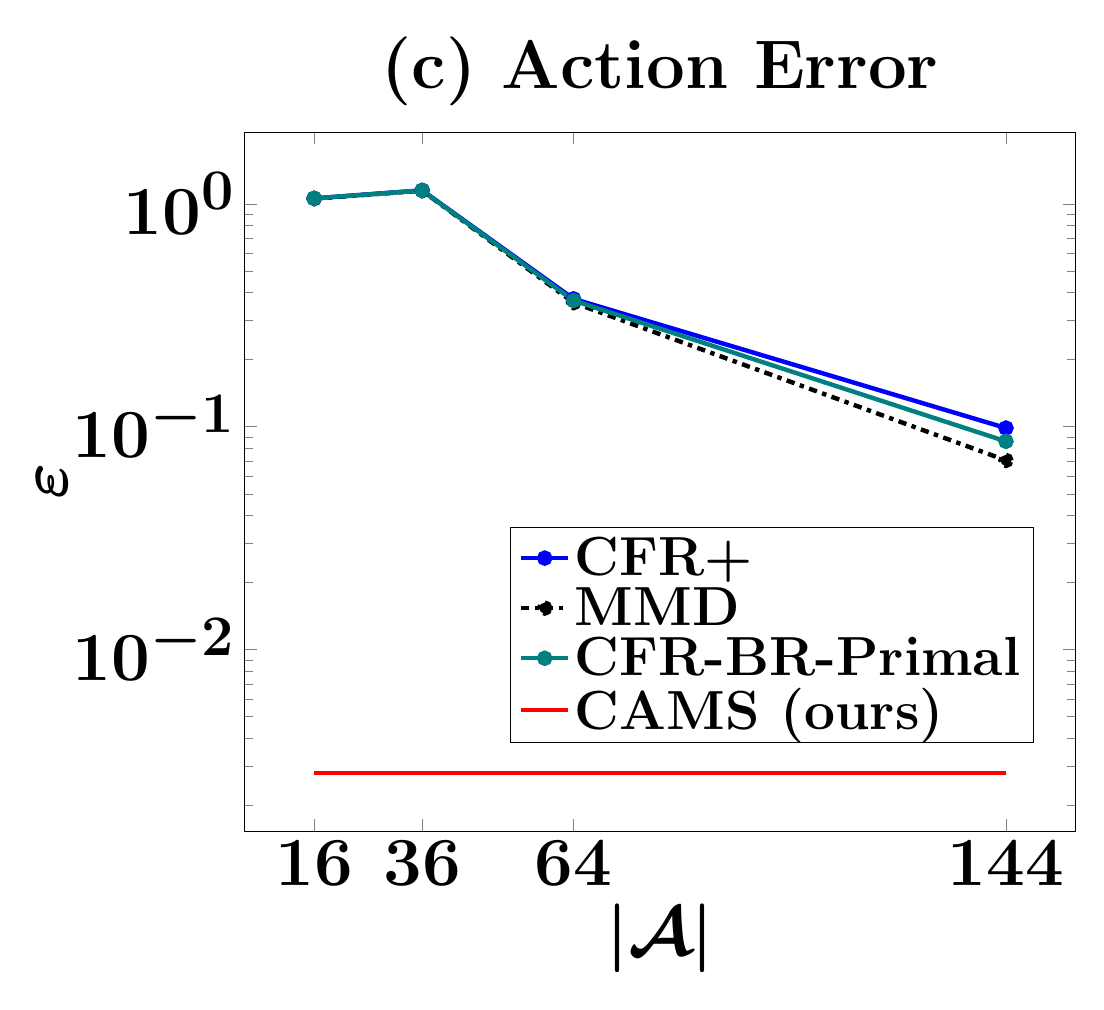
\begin{tikzpicture}[scale=1]
\begin{axis}[title={(c) Action Error},
    legend style={nodes={scale=0.8}, style={at={(0.95, 0.435)}}, fill=none},
    legend cell align={left},
    legend entries={CFR+, MMD, CFR-BR-Primal, CAMS (ours)},
    xlabel={$\boldsymbol{|\mathcal{A}|}$},
    ylabel={$\boldsymbol{\varepsilon}$},
    xtick={16, 36, 64, 144},
    ymode=log,
    ylabel shift=-5pt,
]
% cfr+
\addplot [mark=*, mark size=2pt, ultra thick, blue] coordinates {
(16, 1.0588427800973248)
(36, 1.1494801917079402)
(64, 0.37464195668540257)
(144, 0.09866226893665803)
};
% mmd
% mmd
% [0.5552314866840433,
%  0.5209049957759864,
%  0.5586684894950396,
%  0.6097465051451072]
\addplot[ultra thick, black, mark=*, mark size=2pt, dashdotted] coordinates {
(16, 1.0552507678615948)
(36, 1.146136600348143)
(64, 0.36045590244936615)
(144, 0.07065840307433174)
};
% cfr-br-primal
% 0.6496365514625374,
%  0.2945435474633056,
%  0.1709301707831794,
%  0.03248224069686917
\addplot[ultra thick, mark=*, mark size=2pt, teal] coordinates{
% (16, 0.524)
% (36, 0.568)
% (64, 0.157)
% (144, 0.031)
(16, 1.0581758567678188)
(36, 1.1486716970232314)
(64, 0.3682825954941562)
(144, 0.08599092519673776)
};
% cams
\addplot [ultra thick, red] coordinates {
(16, 0.0028)
(36, 0.0028)
(64, 0.0028)
(144, 0.0028)
};
\end{axis}
\end{tikzpicture}%
\begin{tikzpicture}[scale=1.03]
    \begin{axis}[title={(d) Action Error}, every axis title/.style={above, at={(0.5, 0.986)}},
    legend style={nodes={scale=0.8}, style={at={(0.9, 0.38)}}, fill=none},
    legend cell align={left},
    legend entries={DeepCFR $\boldsymbol{(|\mathcal{A}|=16)}$, DeepCFR $\boldsymbol{(|\mathcal{A}|=9)}$, CAMS (ours)},
    xlabel={$\boldsymbol{t}$},
    ylabel={$\boldsymbol{\bar{\varepsilon}_t}$},
    xtick={0, 0.25, 0.5, 0.75},
    % ytick={0, 5, 10, 15},
    % ymode=log,
    xmax=0.8,
    ylabel shift=-5pt,
]   
% A =16
\addplot [mark=*, mark size=2pt, ultra thick, blue] table[x=x,y=y] {\dcfra};
% A =9
\addplot [mark=*, mark size=2pt, ultra thick, teal] table[x=x,y=y] {\dcfrb};
% cams
\addplot [mark=*, mark size=2pt, ultra thick, red] table[x=x,y=y] {\cams};
% fill betweens
% cfr_9
\addplot [name path=upper,draw=none] table[x=x,y expr=\thisrow{y}+\thisrow{err}] {\dcfrb};
\addplot [name path=lower,draw=none] table[x=x,y expr=\thisrow{y}-\thisrow{err}] {\dcfrb};
\addplot [fill=teal!40, fill opacity=0.4] fill between[of=upper and lower];
% cfr_16
\addplot [name path=upper_2,draw=none] table[x=x,y expr=\thisrow{y}+\thisrow{err}] {\dcfra};
\addplot [name path=lower_2,draw=none] table[x=x,y expr=\thisrow{y}-\thisrow{err}] {\dcfra};
\addplot [fill=blue!40, fill opacity=0.4] fill between[of=upper_2 and lower_2];
% cams
\addplot [name path=upper_3,draw=none] table[x=x,y expr=\thisrow{y}+\thisrow{err}] {\cams};
\addplot [name path=lower_3,draw=none] table[x=x,y expr=\thisrow{y}-\thisrow{err}] {\cams};
\addplot [fill=red!10] fill between[of=upper_3 and lower_3];
    \end{axis}
\end{tikzpicture}
\end{document} 

After collecting diverse trajectories from \texttt{Skill-RRT}, we train an imitation learning (IL) policy for efficient real-world deployment. Although \texttt{Skill-RRT} can be directly deployed in the real world, it is undesirable because planning is time-consuming, and re-planning becomes necessary if unexpected state transitions occur after skill execution. To address this issue, we leverage recent advances in IL, which have demonstrated impressive results in robotic tasks and enable feedforward action prediction \cite{Zhao-RSS-23, chi2023diffusion, Reuss-RSS-23}. For the policy architecture, we specifically adopt Diffusion Policy \cite{chi2023diffusion} to handle the highly multi-modal actions present in the collected trajectories which originate from different subgoals. Note that we only use simulation data—not real-world data—thereby minimizing human effort for data collection across a wide range of initial and goal states.

 
However, we find that training IL policy with entire trajectories from \texttt{Skill-RRT} degrades performance. This happens because some subgoal object poses of skills are not reliable or stable enough to consistently lead to task completion. For example, unstable subgoal object poses positioned very close to the edge of the table might solve the task, but raise the possibility of dropping the card. Training the IL policy with demonstrations prone to such failures leads to a low-performing policy that also exhibits a high probability of failure. Therefore, we improve the quality of trajectories generated by \texttt{Skill-RRT} to achieve high performance of the IL policy \cite{mandlekar2022matters, dalal2023imitating}. We filter out skill plans by replaying them multiple times and discarding plans whose success rate is lower than a threshold. Additionally, we remove trajectories with long time steps within the same skill plan to reduce the time taken to solve the task.

We demonstrate our framework solves three challenging tasks—flipping a card, tiding a book in a bookshelf, and clearing a cup in a kitchen—using non-prehensile (NP) and place (P) skills, without any domain-specific reward design or human demonstration. We also show that the final IL policy can be deployed in the real world in a zero-shot manner with a high success rate. The proposed framework is compared with other approaches including PAMDP and TAMP in Table \ref{table:baseline_comparison}.

Our contribution is summarized as follows:
\begin{enumerate}
  \item \textbf{Effective Skill Chaining}: We demonstrate that our \texttt{Skill-RRT} algorithm can effectively chain a sequence of skills, including contact-rich non-prehensile (NP) skills, without complex modeling of the domain or skills.
  \item \textbf{Skill Acquisition}: We design an abstract version of \texttt{Skill-RRT} to acquire connectors that are necessary to complete the task but are not currently in the skill library.
  \item \textbf{High Performance in Real-World Experiments}: We show that the imitation learning policy achieves high performance in real-world experiments using a simple data filtering mechanism.
\end{enumerate}